%%%%%%%%%%%%%%%%%%%%%%%%%%%%%%%%%%%%%%%%%%%%%%%%%%%%%%%%%%%%%%%%%%%%%%
% Problem statement
\begin{statement}[
  problempoints=70,
  timelimit=2 sekunde,
  memorylimit=512 MiB,
]{Grudanje}

\setlength\intextsep{-0.1cm}
\begin{wrapfigure}[7]{r}{0.25\textwidth}
\centering
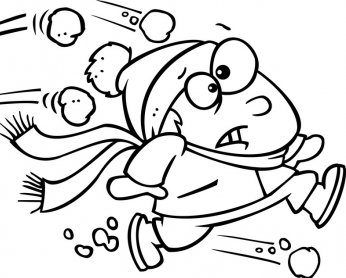
\includegraphics[width=0.25\textwidth]{img/gruda.png}
\end{wrapfigure}

Patrik obožava proučavati riječi hrvatskoga jezika, a posebno mu se sviđaju
riječi koje se sastoje od točno $N$ slova. Kada vidi neku takvu riječ, Patrik
odmah promotri $Q$ njenih podriječi te za svaku podriječ odredi jesu li sva
slova u njoj različita. Ako je to slučaj u svakoj od $Q$ podriječi, tada Patrik
za cijelu riječ kaže da je ona savršena.

Krešimir ne voli proučavati riječi hrvatskoga jezika, već obožava gađati
grudama svog prijatelja Patrika. Jednoga je jutra šetao gradom noseći sa
sobom skrivenih $N$ gruda te je nabasao na Patrika koji je upravo završio s
proučavanjem jedne riječi od $N$ slova koju je neki huligan napisao na zidu.
Kakve li slučajnosti\dots

Krešimir je silovito bacio grudu u smjeru Patrika, ali se ovaj vješto
izmaknuo pa je gruda (umjesto Patrika) pogodila i u potpunosti prekrila $p_1$-vo
slovo riječi na zidu. Na sličan način je Krešimir potrošio i preostalih $(N-1)$
gruda pa je tako njegova $i$-ta bačena gruda pogodila i u potpunosti prekrila
$p_i$-to slovo riječi sa zida. Zanimljivo, nakon što je Krešimiru ponestalo
gruda, cijela je riječ bila prekrivena snijegom.

Patrik je pogledao snijegom prekrivenu riječ te zaključio da je i ona savršena.
Odnosno, proširio je definiciju savršenosti na način da se riječ smatra
savršenom ako niti u jednoj od $Q$ podriječi ne postoje dva slova koja nisu
prekrivena snijegom, a međusobno su jednaka. Sada ga zanima nakon koje je
Krešimirove grude (moguće niti jedne) riječ na zidu postala savršena.

%%%%%%%%%%%%%%%%%%%%%%%%%%%%%%%%%%%%%%%%%%%%%%%%%%%%%%%%%%%%%%%%%%%%%%
% Input
\subsection*{Ulazni podaci}
U prvom je retku riječ koja se sastoji od $N$ $(1 \le N \le 10^5)$ malih slova
engleske abecede.

U drugom je retku prirodan broj $Q$ $(1 \le Q \le 10^5)$ iz teksta zadatka.

U $i$-tom od sljedećih $Q$ redaka su po dva prirodna prirodna broja $a_i$ i
$b_i$ $(1 \le a_i \le b_i \le N)$ koji označavaju da se $i$-ta od $Q$ podriječi iz
teksta zadatka proteže od $a_i$-tog do $b_i$-tog slova riječi sa zida.

U sljedećem se retku nalazi $N$ međusobno različitih prirodnih brojeva $p_i$
$(1 \le p_i \le N)$ iz teksta zadatka.

%%%%%%%%%%%%%%%%%%%%%%%%%%%%%%%%%%%%%%%%%%%%%%%%%%%%%%%%%%%%%%%%%%%%%%
% Output
\subsection*{Izlazni podaci}
U jedini redak ispišite nakon koje je Krešimirove grude riječ na zidu postala
savršena.

%%%%%%%%%%%%%%%%%%%%%%%%%%%%%%%%%%%%%%%%%%%%%%%%%%%%%%%%%%%%%%%%%%%%%%
% Scoring
 \subsection*{Bodovanje}
U test podacima ukupno vrijednima 14 bodova vrijedi $1 \le N, Q \le 500$. \\
U test podacima vrijednima dodatnih 21 bod vrijedi $1 \le N, Q \le 3000$. \\
U test podacima vrijednima dodatnih 14 bodova riječ će se sastojati samo od
slova \texttt{'a'}.


%%%%%%%%%%%%%%%%%%%%%%%%%%%%%%%%%%%%%%%%%%%%%%%%%%%%%%%%%%%%%%%%%%%%%%
% Examples
\subsection*{Probni primjeri}
\begin{tabularx}{\textwidth}{X'X'X}
\sampleinputs{test/grudanje.dummy.in.1}{test/grudanje.dummy.out.1} &
\sampleinputs{test/grudanje.dummy.in.2}{test/grudanje.dummy.out.2} &
\sampleinputs{test/grudanje.dummy.in.3}{test/grudanje.dummy.out.3}
\end{tabularx}

\textbf{Pojašnjenje drugog probnog primjera:}

Nakon 1. grude riječ je: \texttt{abbab*ab} \\
Nakon 2. grude riječ je: \texttt{ab*ab*ab} \\
Nakon 3. grude riječ je: \texttt{ab*a**ab} \\
Nakon 4. grude riječ je: \texttt{*b*a**ab} \\
Nakon 5. grude riječ je: \texttt{*b****ab} \\
Nakon 6. grude riječ je: \texttt{******ab} \\
Nakon 7. grude riječ je: \texttt{*******b} \\
Nakon 8. grude riječ je: \texttt{********}

%%%%%%%%%%%%%%%%%%%%%%%%%%%%%%%%%%%%%%%%%%%%%%%%%%%%%%%%%%%%%%%%%%%%%%
% We're done
\end{statement}

%%% Local Variables:
%%% mode: latex
%%% mode: flyspell
%%% ispell-local-dictionary: "croatian"
%%% TeX-master: "../hio.tex"
%%% End:
